\chapter{Battery 0-5V}\label{ch:Battery voltage conversion}
%**********************************************
\section{Literature}\label{sec:loadcontrol_lit}


\section{Design}\label{sec:loadcontrol_design}

I this design the battery voltage will be go through a signal conditioning process to make it readable from the perspective of an ADC. The ADC we are going to use requires a voltage between 0 and 5V. The battery voltage will vary between 6V and 7.2V if the complete system is working as designed. For the purpose of the design an additional 0.3V will be extended on to either side of the boundaries (5.7V to 7.5V)  Using Op Amps the battery voltage will be designed to vary linearly with an output swing of 3.5V. This 3.5V will be equally spaced from the 0 and 5V boundaries of the ADC (0.75V to 4.25V), the output swing is chosen to be less than 5V in order to prevent possible damage to the ADC in the case that the reconditioned battery voltage exceeds 5V.
\newline 

The immediate problems faced is that the lowest battery voltage is not 0V but rather 5.7V. This means that the battery voltage will require a shift in order for the design requirements above to be met. This is achieved with an inverting op amp with a reference voltage. The voltages as they are will have to to be divided down in order not to breach the differential voltage limits of the MCP op amps that are being used ($|V_{ss}-V_{dd}|$ \cite{MCP}). This can be seen in the voltage following section of figure \ref{fig:batcond}. A voltage follower is used to prevent the negative feedback of the inverting op amp from interfering with the divided battery voltage. The output of the non inverting amplifier is significantly smaller than the requirements. Therefore a non inverting amplifier is then used to amplify this output to required levels.
\newline
To calculate suitable values I worked backwards from the output to the input.
\begin{equation}
V_{out-invert}=2\times V_{invert-ref}+(-1)\times (\frac{R_{F1}}{R_{in1}})\times V_{invert-in}
    \label{eq:invert}
\end{equation}

\begin{equation}
V_{non invert-out}= (1+\frac{R_{F2}}{R_{x}})\times V_{out-invert}
    \label{eq:noninvert}
\end{equation}

The non inverting amplifier is chosen to have a gain of 15. This means that to achieve the output range "0.75V to 4.25V" the non inverting amplifier requires 15 times less than the output "50mV to 283.3mV". Due to using an inverting amplifier the point at which the inverting output is 283.3mV the battery voltage will be 5.7V and when the inverting output is 50mV the battery voltage will be 7.5V. Using eq.\ref{eq:invert} and solving simultaneously for $V_{invert-in}$ ($V_{invert-in}=V_{bat}\times\frac{R_2}{R_2+R_1}$). The inverting amplifier is designed to have unity gain as it only serves the purpose of shifting the battery voltage down. The resistor values are then found to be , $R_1$=180k\textohm \ and $R_2$=27k\textohm. Detailed calculations can be found at appendix \ref{ch:calcA6}. $V_{invert-ref}$ is calculated to be 511mV and is implemented by dividing the 5V regualtor voltage with $R_3$ and $R_4$ (refer to figure \ref{fig:batcond}). 
\newline \newline
To achieve a gain of 15 for the non inverting amplifier (1+$\frac{R_{F2}}{R_{x}}$ from eq.\ref{eq:noninvert}) must be equal to 15. $R_{F2}$ is chosen to be 150k\textohm \ and $R_x$ is calculated to be 10.71k\textohm. Two lab 22k\textohm \ resistors in parallel are used to implement $R_x$ (refer to \ref{fig:batcond}).



\begin{figure}[!htb]
\centering
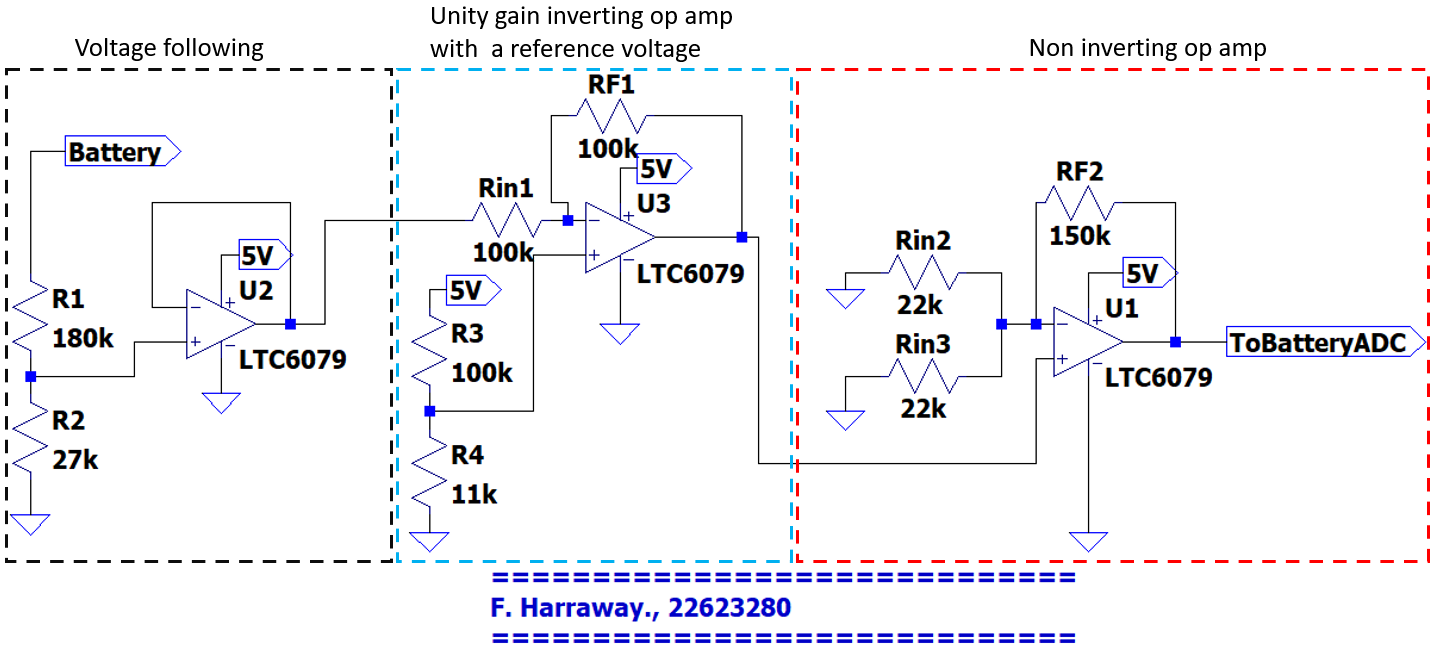
\includegraphics[scale=0.3]{Figures/A6circ1.PNG}
\caption{Battery Voltage Conditioning Circuit}
\label{fig:batcond}
\end{figure}








\section{Results}\label{sec:loadcontrol_results}

\vfill

